\chapter{Diseño e implementación} % Main chapter title
En este capitulo se explica la solución del sistema, tanto desde un punto vista general, como particular, detallando cada una de sus partes.

\section{Arquitectura del sistema}
La arquitectura del trabajo contempla las tres capas de toda aplicación IoT. En la capa física se encuentra la placa ESP32 que centraliza las mediciones de los sensores de humedad ambiente y del sustrato. Dichos datos se envían por Wi-Fi a la capa de transferencia a través un Broker Cloud MQTT. Para establecer la conexión el ESP32 usa los datos de usuario y clave correspondientes del Broker. Luego, al momento de publicar, cada placa enviará sus mensajes a un tópico llamado "\textit{/metrics/<<nodoId>>}", donde \textit{nodoId} es el identificador de la placa en el sistema. De esta manera se realizará la asociación de qué métricas se corresponden con una placa específica. Por otra parte, el Broker disponibilizará la información para el Backend del sistema, que actúa como subscriptor de todos los tópicos mediante "\textit{/metrics/\#}". De esta forma, la capa de presentación obtiene las métricas de cada placa a través de la comunicación con el Backend. Finalmente, el Frontend del sistema permite que los usuarios finales puedan utilizar los datos de sus cultivos. Cada usuario tiene la posibilidad de gestionar su huerta y seleccionar rangos óptimos de aceptación de los porcentajes de humedad. En el caso de tener valores no deseados, el Backend publicará un mensaje en el Broker para dar aviso, a una placa en particular, que realice la apertura de una válvula de agua. Las placas van a recibir los comandos a ejecutar debido a que cada una a esta subscripta al tópico "\textit{/actions/<<suNodoId>>}". En la figura 3.1 se visualiza el diagrama de la arquitectura general del sistema.\\

\begin{figure}[htpb]
\centering 
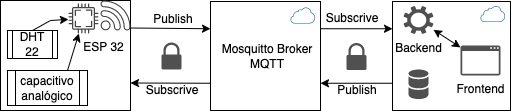
\includegraphics[width=.9\textwidth]{./Figures/arqIoT.png}
\caption{Arquitectura del sistema IoT.}
\label{fig:diagBloques}
\end{figure}

\section{Diseño y arquitectura de la capa física}
Como se menciona en la sección de 'Componentes de hardware' la solución del embebido tiene tres partes fundamentales (placa ESP32, sensor de humedad ambiente y sensor del sustrato). A presar de esto, el diseño del dispositivo, como un todo, es más complejo, ya que se necesitan más componentes para poder operar en el mundo real. A continuación se analiza cada componente y sus conexiones entre si. Esto se puede apreciar en la figura 3.2, diseñada por Damian Reboredo en UNLa [25].


\begin{figure}[htpb]
\centering 
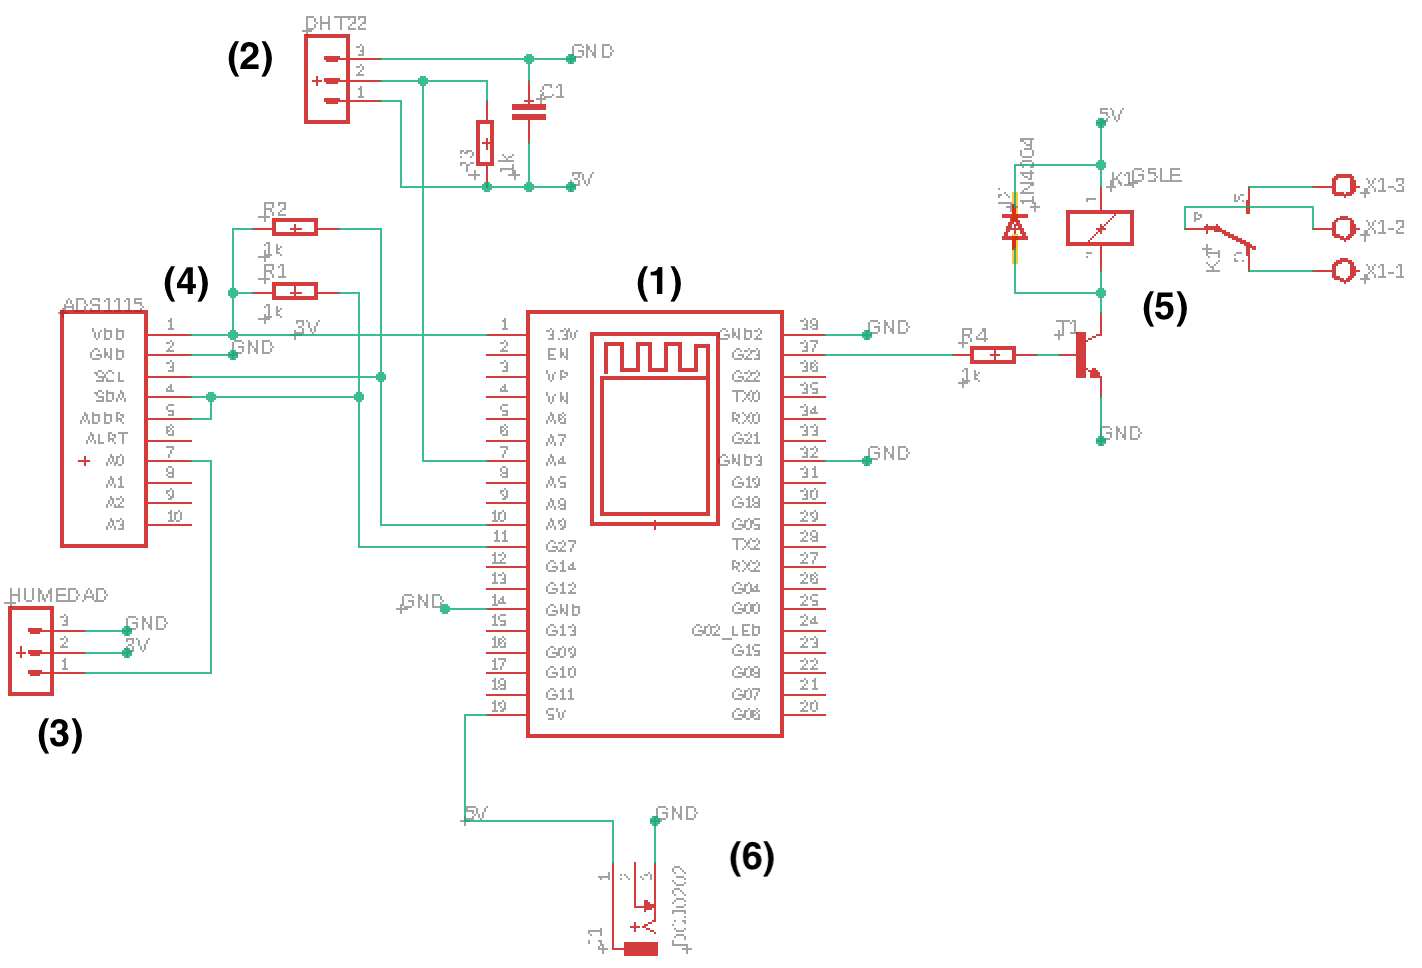
\includegraphics[width=.9\textwidth]{./Figures/diagDipos.png}
\caption{Diagrama del dispositivo.}
\label{fig:diagBloques}
\end{figure}

Como se observa en la imagen, el diseño cuenta con seis secciones importantes.

1. ESP32. Siendo esta la placa que centraliza la información de los sensores, distribuye la energía los componentes. Además, es el componente encargado de enviar los datos vía Wi-Fi. Para lograr esto, dentro contiene la información necesaria para realizar la comunicación con el Bocker MQTT. Además, se encarga de recibir el comando de apertura de la válvula de agua y accionar dicha acción.

2. DHT22. Este sensor realiza la medición la temperatura y humedad ambiente. Es importante resaltar que podría no existir en todos los dispositivos, ya que si en una misma huerta se instalan entre dos y cuatro placas ESP32, solo una llevará el rol de medición de humedad ambiente. Esto último se debe tener en cuenta a la hora de realizar el plano de la huerta. Por otro lado, la programación del ESP32 tiene que estar preparada para contar o no con este sensor.

3. Sensor de humedad del sustrato. A diferencia del sensor DHT22, este está presente en cada una de las ESP2 de la huerta. En todos los casos se usa este componente para validar la humedad relativa del suelo en un conjunto de cultivos.

4. ADS1115. Se utiliza este componente para cambiar la señal analógica del sensor de humedad del sustrato a digital. De esta forma se genera la interacción de información con la placa ESP32.

5. Válvula de agua. En este caso, como se puede ver en el diagrama, se armó el prototipo para accionar un relé. De esta forma se simula la acción de apertura de una manguera. Para el trabajo final se cambia esto último para trabajar con la válvula.

6. Fuente de alimentación. Para este punto, como en el anterior, se pensó inicialmente una fuente directa. Para el caso del producto final de este trabajo se cambia este enfoque hacia el uso de una batería. De esta manera se quiere prescindir de la existencia de un cableado de corriente eléctrica.\\ \\

%----------------------------------------------------------------------------------------

\section{Arquitectura integración del Backend con el Broker MQTT}

Para simplificar la capa de integración con el Broker MQTT se definió crear un servicio con NodeJS que funcione como un \textit{Cron Job}. De esta forma este desarrollo tiene la responsabilidad de obtener la información publicada en el Broker, procesarla y persistirla en la base de datos. Luego, la aplicación en Java Spring queda con la responsabilidad de ejecutar la lógica de negocio del sistema y exponer la API Rest para consumo del Frontend. En la imagen 3.3 se puede observar el diagrama de la arquitectura descripta.\\

\begin{figure}[htpb]
\centering 
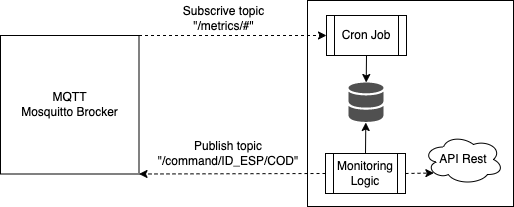
\includegraphics[width=.9\textwidth]{./Figures/arqBE.png}
\caption{Arquitectura backend e integración con Mosquitto del dispositivo.}
\label{fig:diagBloques}
\end{figure}

%----------------------------------------------------------------------------------------

\section{Desarrollo base del Backend y Frontend en UNLa}
Por parte de la capa lógica, Luciano Otegui y Guido Contento hicieron foco en generar la base del Backend y del Frontend para el trabajo. Se realizó el armado de casos de uso y diagrama de clases. Por otra parte, crearon la estructura mínima del sistema para una correcta interacción de usuarios finales. Finalmente, se definieron las vistas y estilos generales del sitio. Al igual que el caso anterior, el código base del backend [26] y del frontend [27] se alojaron en repositorios del dominio de la universidad.\\

%----------------------------------------------------------------------------------------

\section{Despliegue del sistema en UNLa}

Para la puesta en producción se va a construir una huerta en uno de los predios de la UNLa. Para esto se van a seguir las especificaciones de la figura 3.4. Como se puede apreciar, se van a armar seis kits de dispositivos para tomar mediciones. De estos, solo uno tendrá el sensor DHT22, y todos contarán con el sensor de humedad del sustrato. En la imagen se observa unas líneas de color azul, estas representan la cañería de agua. Este montaje se llevará en conjunto con el equipo de mantenimiento de la UNLa y será destinado para probar el trabajo, así como también, para realizar muestras a estudiante y visitantes en la universidad.

\begin{figure}[htpb]
\centering 
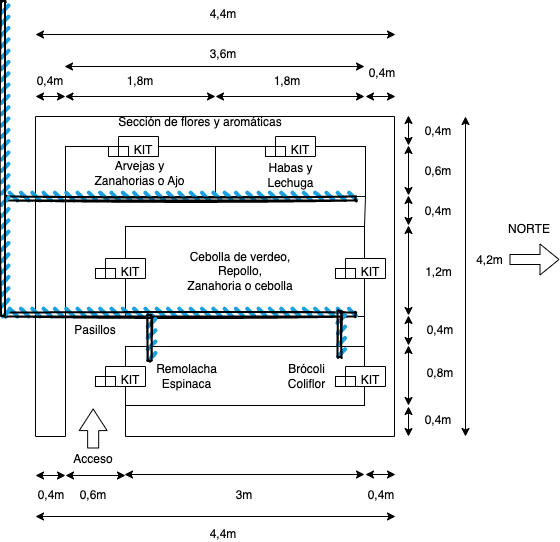
\includegraphics[width=.7\textwidth]{./Figures/despliegue.png}
\caption{Mapa de la huerta en UNLa.}
\label{fig:diagBloques}
\end{figure}

%----------------------------------------------------------------------------------------
